

\documentclass{beamer}
\usepackage{HECbeamer}
% \usepackage{pgfpages}
% \pgfpagesuselayout{4 on 1}[letterpaper, landscape, border shrink=5mm]
\title[\color{white}{MATH 60604A \S~4g - Log-linear models with offset}]{\texorpdfstring{MATH 60604A \\Statistical modelling \\ \S~4g - Log-linear models with offset}{MATH 60604A \\Statistical modelling \\ \S~4g - Log-linear models with offset}}
\author{}
\institute{HEC Montréal\\
Department of Decision Sciences}
\date{} 

\begin{document}
\frame{\titlepage}



\begin{frame}[fragile]
\frametitle{Offsets and comparison of counts}
\bi
\item Up to now, we implicitly assumed that the the count variables $Y$ were \alert{comparable} between observations.
\bi 
\item In the fixation example, $Y_i$ represented the number of times that subject $i$ bought the product in the month following the study completion.
\ei
\item What if the period of follow-up varied from one individual to another?
\bi
\item the number of work accidents seen in a business in a given time period depends on the number of its employees.
\item the number of cancer incidence per region depends on the number of inhabitants.
\ei
\ei
If the counts are not comparable, we can compare the \textbf{rates} instead (number of purchases per month, number of accident per employee, etc.)


If we model rates with the Poisson model, the latter is adequate \textbf{only} if the rate is \alert{small}.

\end{frame}
% 
% \begin{frame}[fragile]
% \frametitle{Making the counts comparable}
% \bi
% \item In all these examples, the variable $Y$ is not comparable between subject (between lines of the data file)
% \item Talking about the ``number of\ldots'' doesn't mean anything if we don't know the follow-up time of the subject, the number of employees in a business, the size of the cookie, etc.
% \item Instead, we can talk about a \alert{rate}:
% \bi
% 
% \item The rate of purchase (number of purchases per month)
% \item The work accident rate (number of accidents per employee)
% \item The chocolate chip rate (number of chocolate chips per square centimetre of a cookie)
% \ei
% \ei
% \end{frame}

\begin{frame}[fragile]
\frametitle{Car accident example}
The National Highway Traffic Safety Administration (NHTSA) compiles statistics about road traffic deaths in the Fatality Analysis Reporting System. The yearly mortality counts for $2010$ and $2018$ are given in \code{crash}  according to whether the accident occured during daytime or nighttime (\code{time}), and according to the NHTSA-defined geographic area (\code{region}).

\bi
\item Let $Y_i$ denotes the number of death in a given year in region $i$;
\item Let $N_i$ denotes the number of inhabitants in region $i$.
\ei
The goal is to estimate the relationship between the number of fatal car crash and timing of the incident.
\end{frame}
\begin{frame}
 \begin{center}
  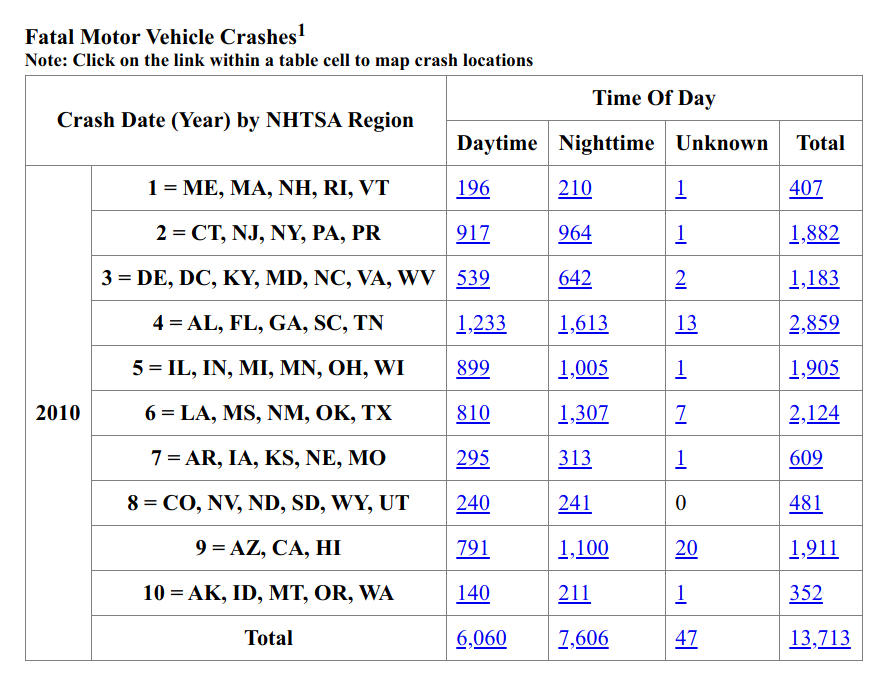
\includegraphics[width = 0.6\linewidth]{img/c4/crash.png}
 \end{center}
\end{frame}


\begin{frame}[fragile]
\frametitle{Car accident example}
\bi
\item If we ignore the size of the population, the Poisson regression model (or negative binomial) would be
\begin{align*}
\ln(\mu_i)=\ln\{\E{Y_i}\}=\beta_0 + \beta_1 \code{time} + \beta_2 \code{year}
\end{align*}
\item If we want to account for the size of the population in a given region, we would model $Y_i/N_i$ instead of $Y_i$.
\item This amounts to setting 
\begin{align*}
\ln\left\{\frac{\E{Y_i}}{N_i}\right\}&=\beta_0 +\beta_1 \code{time} + \beta_2 \code{year}
\intertext{or equivalently}
\ln\left\{\E{Y_i}\right\}&=\beta_0 + \beta_1 \code{time} + \beta_2 \code{year}+\ln( N_i)
\end{align*}
\item The term $\ln(N_i)$ is called an \alert{\textbf{offset}} since it is included as a covariate, but there is no $\beta$ coefficient to estimate (unity).
\ei
\end{frame}

\begin{frame}[fragile]
\frametitle{Car accident}

\begin{tcolorbox}[colback=white, colframe=hecblue, title=\SASlang{} code to include an offset term]
{\small
\begin{verbatim}
data crash;
set statmod.crash;
logpopn=log(popn);
run;

proc genmod data=crash;
class time(ref="day") year(ref="2010");
model ndeath=time year / dist=negbin link=log 
    offset=logpopn type3 lrci;
run;
\end{verbatim}
}
\end{tcolorbox}
{\footnotesize 

The option \texttt{offset} could also be included for a Poisson model.



}
\begin{center}
 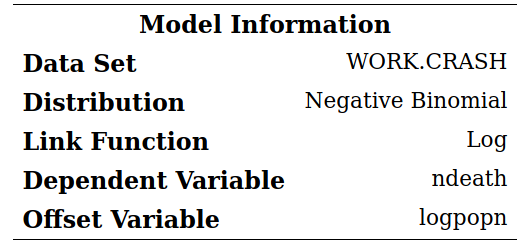
\includegraphics[width = 0.4\linewidth]{img/c4/slides8-e9}
\end{center}

\end{frame}
\begin{frame}{Parameter interpretation with offset}
\begin{center}
 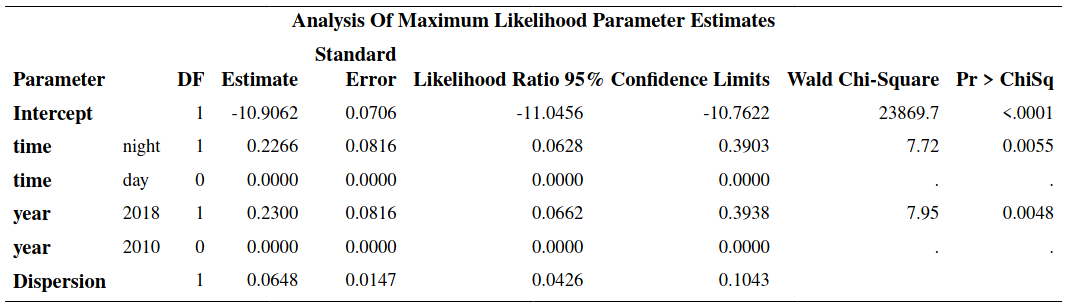
\includegraphics[width = 0.99\linewidth]{img/c4/slides8-e10}
\end{center}
{\small 
\bi \item Since the variable $\ln(N)$ is included as an offset, it doesn't appear in the table.
\item The deviance statistic (output not shown) is $40.269$ for $37$ degrees of freedom (ratio of $1.0884$). The corresponding $p$-value is $0.327$, so there is no evidence that our fitted model is inadequate.
\item In this setting, $\exp(\hat{\beta}_0)=\exp(-10.9062)$ corresponds to the estimated mortality rate during daytime in $2010$, which is $1.83/100000$, i.e., a rate of $1.83$ per $100\,000$ inhabitants (with 95\% confidence interval [$1.60  \times 10^{-5}, 2.12 \times 10^{-5}]$).
\item There is a $\exp(0.23)$ change in mortality from $2010$ to $2018$, corresponding to a $26$\% increase in road casualties.
\ei
}
\end{frame}
\end{document}
